\documentclass[conference]{IEEEtran}
\usepackage{amsmath,booktabs,graphicx}
\title{Comparing Attention-Pooled Recurrent Networks for IMDb Sentiment Classification}

\author{
\IEEEauthorblockN{Nicholas Ampimah and Jane Ohia}
\IEEEauthorblockA{University of Nebraska--Lincoln}
}

\begin{document}
\maketitle

\begin{abstract}
We compare bidirectional gated recurrent unit (BiGRU) and long short-term memory (BiLSTM) models for binary sentiment classification of IMDb movie reviews. Both architectures use learned embeddings, masked attention pooling, and dropout regularization, with dropout rates of 0.20 and 0.50, yielding four models. A stratified validation split is used for early stopping and model selection, while the official test split remains held out. BiLSTM-A, selected by minimum validation cross-entropy, achieved 84.84\% test accuracy, 0.848 macro-F1, and 15.16\% error with a 95\% Wilson confidence interval of 14.72--15.61\%. Increasing dropout to 0.50 worsened minimum validation loss for both recurrent architectures and did not eliminate overfitting.
\end{abstract}

\begin{IEEEkeywords}
sentiment analysis, IMDb, recurrent neural networks, attention, dropout
\end{IEEEkeywords}

\section{Introduction}
Sentiment analysis maps text to an opinion label and is naturally sequential because word order, negation, and long-range context can change meaning. We study the 50,000-review IMDb benchmark \cite{maas} using two bidirectional recurrent encoders: BiGRU and BiLSTM. Both are paired with the same masked attention and classifier head so that the recurrent cell is the main architectural difference. Within each architecture, dropout is varied from 0.20 to 0.50 to test whether stronger regularization improves generalization. BiLSTM-A achieved the lowest validation loss, 0.3027, and was therefore selected before test evaluation. It reached 84.84\% test accuracy. The four test accuracies differed by only 0.31 percentage points, and stronger dropout did not improve validation loss or prevent overfitting.

\section{Problem, Data, and Models}
\subsection{Learning Problem and Data}
The input is a movie review represented by at most 200 token IDs, and the output is the probability $p_\theta(y=1\mid x)$ that the review is positive, where $y\in\{0,1\}$. A threshold of 0.5 produces the negative/positive prediction. Training minimizes binary cross-entropy,
\begin{equation}
\mathcal{L}=-\frac{1}{B}\sum_{i=1}^{B}
[y_i\log p_i+(1-y_i)\log(1-p_i)].
\end{equation}
Cross-entropy is appropriate because the task is binary probabilistic classification and penalizes confident incorrect predictions.

TensorFlow Datasets provides 25,000 training and 25,000 test reviews. Using seed 42, the official training set is stratified into 20,000 training and 5,000 validation reviews. The official test split is not used for architecture or hyperparameter selection. Text is lowercased; HTML line breaks and most punctuation are removed while apostrophes are retained. A vocabulary of at most 15,000 tokens is fitted only on the training reviews. Reviews are padded or truncated to 200 tokens to bound recurrent computation, with the limitation that late sentiment evidence can be lost.

\subsection{Architectures and Training}
Each token is mapped to a 64-dimensional learned embedding. The encoder is either a bidirectional GRU or bidirectional LSTM with 48 units per direction, producing a $200\times96$ sequence of contextual states. Bidirectionality is appropriate because the complete review is available at inference and sentiment can depend on both preceding and following context.

Masked attention computes
\begin{equation}
s_t=v^\top\tanh(Wh_t+b), \qquad
\alpha_t=\frac{e^{s_t}}{\sum_j e^{s_j}},
\end{equation}
over nonpadding positions and returns $\sum_t\alpha_t h_t$. This allows the classifier to emphasize informative positions instead of relying only on the final recurrent state. The pooled vector passes through a 32-unit ReLU layer, dropout, and a sigmoid output. Setting A uses dropout 0.20 and setting B uses 0.50; thus four models are evaluated. Dropout is used to reduce co-adaptation and overfitting.

All models use Adam with learning rate $10^{-3}$ and batch size 128. Early stopping monitors validation loss with patience 5 and restores the best checkpoint. The actual run used a 300-epoch safety cap, but all models stopped after the required non-improvement window. Model selection was frozen before the official test set was scored.

\begin{table*}[t]
\caption{Validation-selected checkpoints and held-out test performance. $^\ast$ indicates the model selected by minimum validation loss. Error intervals are 95\% Wilson confidence intervals.}
\label{tab:results}
\centering
\small
\setlength{\tabcolsep}{4.2pt}
\begin{tabular}{lccccccc}
\toprule
Model & Best/Stop & Dropout & Val. Loss & Accuracy (\%) & Macro-F1 & ROC AUC & Error (\%) [95\% CI] \\
\midrule
BiGRU-A & 2/7 & 0.20 & 0.3040 & 85.06 & 0.850 & 0.931 & 14.94 [14.51, 15.39] \\
BiGRU-B & 2/7 & 0.50 & 0.3055 & 85.10 & 0.851 & 0.930 & 14.90 [14.47, 15.35] \\
BiLSTM-A$^\ast$ & 2/7 & 0.20 & \textbf{0.3027} & 84.84 & 0.848 & 0.930 & 15.16 [14.72, 15.61] \\
BiLSTM-B & 1/6 & 0.50 & 0.3179 & 85.15 & 0.851 & 0.930 & 14.85 [14.41, 15.29] \\
\bottomrule
\end{tabular}
\end{table*}

\section{Results and Discussion}
\subsection{Performance and Model Selection}
Table~\ref{tab:results} compares validation loss, accuracy, macro-F1, ROC AUC, and generalization error. Accuracy measures overall correctness, macro-F1 gives equal weight to positive and negative classes, and ROC AUC evaluates ranking quality across thresholds. For $k$ errors among $n$ independent test examples, the error rate is $\hat e=k/n$; 95\% Wilson intervals quantify test-sample uncertainty in this generalization-error estimate.

BiLSTM-A was selected because its validation loss, 0.3027, was the lowest of the four models. BiLSTM-B had the highest observed test accuracy, 85.15\%, but its worse validation loss, 0.3179, cannot be used retroactively to replace the validation-selected model. This separation of validation-based selection from final testing prevents test-set leakage. The overlapping confidence intervals also show that the small observed test differences should not be interpreted as strong evidence that one model is statistically superior.

\begin{figure*}[t]
\centering
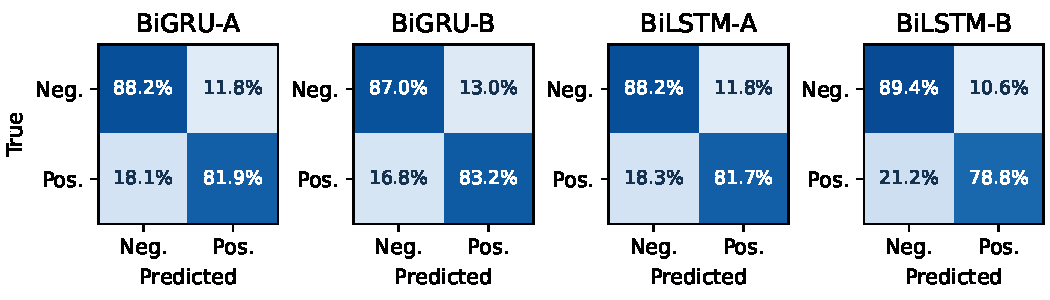
\includegraphics[width=0.82\textwidth]{results/confusion_matrices.pdf}
\caption{Row-normalized confusion matrices on the 25,000-review test set. Rows are true classes and columns are predicted classes.}
\label{fig:cm}
\end{figure*}

\subsection{Confusion Matrices, Dropout, and Overfitting}
Figure~\ref{fig:cm} gives the required normalized confusion matrices. All four models classified negative reviews somewhat better than positive reviews. For BiLSTM-A, positive recall was 81.38\% and negative recall was 88.30\%, corresponding to 2,327 false negatives and 1,462 false positives.

Increasing dropout from 0.20 to 0.50 changed minimum validation loss from 0.3040 to 0.3055 for BiGRU and from 0.3027 to 0.3179 for BiLSTM. Thus stronger dropout did not improve validation performance in either architecture. The training histories also show overfitting after the best checkpoint: for BiLSTM-A, training loss decreased from 0.2333 at epoch 2 to 0.0331 at epoch 7 while validation loss increased from 0.3027 to 0.6572. Early stopping was therefore important for retaining the best-generalizing weights.

\section{Strengths and Limitations}
The experiment uses identical preprocessing, data partitions, attention, classifier layers, optimizer settings, and selection criteria across models, supporting a controlled comparison. The held-out test set is isolated from model selection, and normalized confusion matrices and confidence intervals provide more information than accuracy alone. Limitations include a single split and seed, different parameter counts for GRU and LSTM, possible information loss from truncating reviews to 200 tokens, and the fact that attention weights are not causal explanations. Results are specific to polarized IMDb reviews and may not transfer directly to neutral sentiment or other domains.

\section{Conclusion}
BiLSTM-A was selected by minimum validation cross-entropy and achieved 84.84\% test accuracy, 0.848 macro-F1, and 15.16\% error with a 95\% Wilson interval of 14.72--15.61\%. Dropout 0.50 did not improve minimum validation loss for either recurrent architecture, and all models showed overfitting after their best checkpoint. Overall, masked attention with bidirectional recurrent encoders provided similar held-out performance across the four tested configurations, while validation-based selection and early stopping were essential for a defensible comparison.

\begin{thebibliography}{1}
\bibitem{maas}
A.~L. Maas \emph{et al.}, ``Learning word vectors for sentiment analysis,'' in \emph{Proc. ACL-HLT}, 2011, pp. 142--150.
\end{thebibliography}

\end{document}
